%%===========================================================%%
%%                                                           %%
%%                       EFFICIENCIES                        %%
%%                                                           %%
%%===========================================================%%


\chapter{Efficiencies}\label{chap:efficiencies}

\section{TPC track acceptance and reconstruction efficiency}\label{sec:tpcRecoEff}
We define joint acceptance and efficiency of the reconstruction of a track in the TPC, $\epsilon_{\textrm{\tiny TPC}}$, as the probability that particle from the primary interaction generates signal in the detector which is reconstructed as a track that satisfies all quality criteria and whose $p_{T}$ and $\eta$ are within the kinematic region of the measurement (cuts~\ref{enum:TpcKinematicCuts} and ~\ref{enum:TpcQualityCuts}).

Thechnically this quantity is derived from STARsim MC embedded into zero-bias triggers in the following procedure:
\begin{enumerate}
	\item True-level primary particles of given ID and charge, with all physics ($p_{T}^{\textrm{true}}$, $\eta^{\textrm{true}}$) and detector ($z_{\textrm{vx}}$) quantities within defined region of the measurement, are selected ($set~A$).
	\item Each particle from $set~A$ is checked if global TPC track with more than half of hit points generated by this particle, was reconstructed. All global tracks which are associated with true-level primary particles and satisfy kinematic and quality criteria (cuts~\ref{enum:TpcKinematicCuts} and ~\ref{enum:TpcQualityCuts}), form $set~B$.
	\item The joint TPC acceptance and efficiency is calculated as the ratio of the histograms of true-level quantities (such as $p_{T}$, $\eta$, $z_{\textrm{vx}}$) for particles from $set~B$ and particles from $set~A$:
	\begin{equation}\label{eq:tpcAccAndEffDefinition}
		\epsilon_{\textrm{\tiny TPC}}\left(p_{T}, \eta, z_{vx};~\textrm{sign},\textrm{PID}\right) = \frac{(p_{T},\eta, z_{vx})~\textrm{histogram for particles of given sign and ID from}~set~B}{(p_{T},\eta, z_{vx})~\textrm{histogram for particles of given sign and ID from}~set~A}.
	\end{equation}

\end{enumerate}


%---------------------------
\begin{figure}[hb]
\caption[TPC acceptance and reconstruction efficiency of $\pi^{-}$.]{TPC acceptance and reconstruction efficiency of $\pi^{-}$. Each plot represents the TPC efficiency $\epsilon_{\text{TPC}}$ ($z$-axis) as a function of true particle pseudorapidity $\eta$ ($x$-axis) and transverse momentum $p_{T}$ ($y$-axis) in single $z$-vertex bin whose range is given at the top. Red lines and arrows indicate region accepted in analyses.}\label{fig:eff_pion_minus}
\centering
\parbox{0.495\textwidth}{
  \centering
  \includegraphics[width=\linewidth,page=3]{graphics/eff/Eff2D_TPC_pion_Minus.pdf}\\
  \includegraphics[width=\linewidth,page=5]{graphics/eff/Eff2D_TPC_pion_Minus.pdf}\\
  \includegraphics[width=\linewidth,page=7]{graphics/eff/Eff2D_TPC_pion_Minus.pdf}\\
  \includegraphics[width=\linewidth,page=9]{graphics/eff/Eff2D_TPC_pion_Minus.pdf}
}~
\parbox{0.495\textwidth}{
  \centering
  \includegraphics[width=\linewidth,page=4]{graphics/eff/Eff2D_TPC_pion_Minus.pdf}\\
  \includegraphics[width=\linewidth,page=6]{graphics/eff/Eff2D_TPC_pion_Minus.pdf}\\
  \includegraphics[width=\linewidth,page=8]{graphics/eff/Eff2D_TPC_pion_Minus.pdf}\\
  \includegraphics[width=\linewidth,page=10]{graphics/eff/Eff2D_TPC_pion_Minus.pdf}
}%
\end{figure}
\begin{figure}[hb]\ContinuedFloat
% ~\\[32pt]
\centering
\parbox{0.495\textwidth}{
  \centering
  \includegraphics[width=\linewidth,page=11]{graphics/eff/Eff2D_TPC_pion_Minus.pdf}\\
  \includegraphics[width=\linewidth,page=13]{graphics/eff/Eff2D_TPC_pion_Minus.pdf}\\
  \includegraphics[width=\linewidth,page=15]{graphics/eff/Eff2D_TPC_pion_Minus.pdf}\\
  \includegraphics[width=\linewidth,page=17]{graphics/eff/Eff2D_TPC_pion_Minus.pdf}
}~
\parbox{0.495\textwidth}{
  \centering
  \includegraphics[width=\linewidth,page=12]{graphics/eff/Eff2D_TPC_pion_Minus.pdf}\\
  \includegraphics[width=\linewidth,page=14]{graphics/eff/Eff2D_TPC_pion_Minus.pdf}\\
  \includegraphics[width=\linewidth,page=16]{graphics/eff/Eff2D_TPC_pion_Minus.pdf}\\
  \includegraphics[width=\linewidth,page=18]{graphics/eff/Eff2D_TPC_pion_Minus.pdf}
}%
\end{figure}
%---------------------------


%---------------------------
\begin{figure}[hb]
\caption[TPC acceptance and reconstruction efficiency of $\pi^{+}$.]{TPC acceptance and reconstruction efficiency of $\pi^{+}$. Each plot represents the TPC efficiency $\epsilon_{\text{TPC}}$ ($z$-axis) as a function of true particle pseudorapidity $\eta$ ($x$-axis) and transverse momentum $p_{T}$ ($y$-axis) in single $z$-vertex bin whose range is given at the top. Red lines and arrows indicate region accepted in analyses.}\label{fig:eff_pion_plus}
\centering
\parbox{0.495\textwidth}{
  \centering
  \includegraphics[width=\linewidth,page=3]{graphics/eff/Eff2D_TPC_pion_Plus.pdf}\\
  \includegraphics[width=\linewidth,page=5]{graphics/eff/Eff2D_TPC_pion_Plus.pdf}\\
  \includegraphics[width=\linewidth,page=7]{graphics/eff/Eff2D_TPC_pion_Plus.pdf}\\
  \includegraphics[width=\linewidth,page=9]{graphics/eff/Eff2D_TPC_pion_Plus.pdf}
}~
\parbox{0.495\textwidth}{
  \centering
  \includegraphics[width=\linewidth,page=4]{graphics/eff/Eff2D_TPC_pion_Plus.pdf}\\
  \includegraphics[width=\linewidth,page=6]{graphics/eff/Eff2D_TPC_pion_Plus.pdf}\\
  \includegraphics[width=\linewidth,page=8]{graphics/eff/Eff2D_TPC_pion_Plus.pdf}\\
  \includegraphics[width=\linewidth,page=10]{graphics/eff/Eff2D_TPC_pion_Plus.pdf}
}%
\end{figure}
\begin{figure}[hb]\ContinuedFloat
% ~\\[32pt]
\centering
\parbox{0.495\textwidth}{
  \centering
  \includegraphics[width=\linewidth,page=11]{graphics/eff/Eff2D_TPC_pion_Plus.pdf}\\
  \includegraphics[width=\linewidth,page=13]{graphics/eff/Eff2D_TPC_pion_Plus.pdf}\\
  \includegraphics[width=\linewidth,page=15]{graphics/eff/Eff2D_TPC_pion_Plus.pdf}\\
  \includegraphics[width=\linewidth,page=17]{graphics/eff/Eff2D_TPC_pion_Plus.pdf}
}~
\parbox{0.495\textwidth}{
  \centering
  \includegraphics[width=\linewidth,page=12]{graphics/eff/Eff2D_TPC_pion_Plus.pdf}\\
  \includegraphics[width=\linewidth,page=14]{graphics/eff/Eff2D_TPC_pion_Plus.pdf}\\
  \includegraphics[width=\linewidth,page=16]{graphics/eff/Eff2D_TPC_pion_Plus.pdf}\\
  \includegraphics[width=\linewidth,page=18]{graphics/eff/Eff2D_TPC_pion_Plus.pdf}
}%
\end{figure}
%---------------------------





%---------------------------
\begin{figure}[hb]
\caption[TPC acceptance and reconstruction efficiency of $K^{-}$.]{TPC acceptance and reconstruction efficiency of $K^{-}$. Each plot represents the TPC efficiency $\epsilon_{\text{TPC}}$ ($z$-axis) as a function of true particle pseudorapidity $\eta$ ($x$-axis) and transverse momentum $p_{T}$ ($y$-axis) in single $z$-vertex bin whose range is given at the top. Red lines and arrows indicate region accepted in analyses.}\label{fig:eff_kaon_minus}
\centering
\parbox{0.495\textwidth}{
  \centering
  \includegraphics[width=\linewidth,page=3]{graphics/eff/Eff2D_TPC_kaon_Minus.pdf}\\
  \includegraphics[width=\linewidth,page=5]{graphics/eff/Eff2D_TPC_kaon_Minus.pdf}\\
  \includegraphics[width=\linewidth,page=7]{graphics/eff/Eff2D_TPC_kaon_Minus.pdf}\\
  \includegraphics[width=\linewidth,page=9]{graphics/eff/Eff2D_TPC_kaon_Minus.pdf}
}~
\parbox{0.495\textwidth}{
  \centering
  \includegraphics[width=\linewidth,page=4]{graphics/eff/Eff2D_TPC_kaon_Minus.pdf}\\
  \includegraphics[width=\linewidth,page=6]{graphics/eff/Eff2D_TPC_kaon_Minus.pdf}\\
  \includegraphics[width=\linewidth,page=8]{graphics/eff/Eff2D_TPC_kaon_Minus.pdf}\\
  \includegraphics[width=\linewidth,page=10]{graphics/eff/Eff2D_TPC_kaon_Minus.pdf}
}%
\end{figure}
\begin{figure}[hb]\ContinuedFloat
% ~\\[32pt]
\centering
\parbox{0.495\textwidth}{
  \centering
  \includegraphics[width=\linewidth,page=11]{graphics/eff/Eff2D_TPC_kaon_Minus.pdf}\\
  \includegraphics[width=\linewidth,page=13]{graphics/eff/Eff2D_TPC_kaon_Minus.pdf}\\
  \includegraphics[width=\linewidth,page=15]{graphics/eff/Eff2D_TPC_kaon_Minus.pdf}\\
  \includegraphics[width=\linewidth,page=17]{graphics/eff/Eff2D_TPC_kaon_Minus.pdf}
}~
\parbox{0.495\textwidth}{
  \centering
  \includegraphics[width=\linewidth,page=12]{graphics/eff/Eff2D_TPC_kaon_Minus.pdf}\\
  \includegraphics[width=\linewidth,page=14]{graphics/eff/Eff2D_TPC_kaon_Minus.pdf}\\
  \includegraphics[width=\linewidth,page=16]{graphics/eff/Eff2D_TPC_kaon_Minus.pdf}\\
  \includegraphics[width=\linewidth,page=18]{graphics/eff/Eff2D_TPC_kaon_Minus.pdf}
}%
\end{figure}
%---------------------------


%---------------------------
\begin{figure}[hb]
\caption[TPC acceptance and reconstruction efficiency of $K^{+}$.]{TPC acceptance and reconstruction efficiency of $K^{+}$. Each plot represents the TPC efficiency $\epsilon_{\text{TPC}}$ ($z$-axis) as a function of true particle pseudorapidity $\eta$ ($x$-axis) and transverse momentum $p_{T}$ ($y$-axis) in single $z$-vertex bin whose range is given at the top. Red lines and arrows indicate region accepted in analyses.}\label{fig:eff_kaon_plus}
\centering
\parbox{0.495\textwidth}{
  \centering
  \includegraphics[width=\linewidth,page=3]{graphics/eff/Eff2D_TPC_kaon_Plus.pdf}\\
  \includegraphics[width=\linewidth,page=5]{graphics/eff/Eff2D_TPC_kaon_Plus.pdf}\\
  \includegraphics[width=\linewidth,page=7]{graphics/eff/Eff2D_TPC_kaon_Plus.pdf}\\
  \includegraphics[width=\linewidth,page=9]{graphics/eff/Eff2D_TPC_kaon_Plus.pdf}
}~
\parbox{0.495\textwidth}{
  \centering
  \includegraphics[width=\linewidth,page=4]{graphics/eff/Eff2D_TPC_kaon_Plus.pdf}\\
  \includegraphics[width=\linewidth,page=6]{graphics/eff/Eff2D_TPC_kaon_Plus.pdf}\\
  \includegraphics[width=\linewidth,page=8]{graphics/eff/Eff2D_TPC_kaon_Plus.pdf}\\
  \includegraphics[width=\linewidth,page=10]{graphics/eff/Eff2D_TPC_kaon_Plus.pdf}
}%
\end{figure}
\begin{figure}[hb]\ContinuedFloat
% ~\\[32pt]
\centering
\parbox{0.495\textwidth}{
  \centering
  \includegraphics[width=\linewidth,page=11]{graphics/eff/Eff2D_TPC_kaon_Plus.pdf}\\
  \includegraphics[width=\linewidth,page=13]{graphics/eff/Eff2D_TPC_kaon_Plus.pdf}\\
  \includegraphics[width=\linewidth,page=15]{graphics/eff/Eff2D_TPC_kaon_Plus.pdf}\\
  \includegraphics[width=\linewidth,page=17]{graphics/eff/Eff2D_TPC_kaon_Plus.pdf}
}~
\parbox{0.495\textwidth}{
  \centering
  \includegraphics[width=\linewidth,page=12]{graphics/eff/Eff2D_TPC_kaon_Plus.pdf}\\
  \includegraphics[width=\linewidth,page=14]{graphics/eff/Eff2D_TPC_kaon_Plus.pdf}\\
  \includegraphics[width=\linewidth,page=16]{graphics/eff/Eff2D_TPC_kaon_Plus.pdf}\\
  \includegraphics[width=\linewidth,page=18]{graphics/eff/Eff2D_TPC_kaon_Plus.pdf}
}%
\end{figure}
%---------------------------













%---------------------------
\begin{figure}[hb]
\caption[TPC acceptance and reconstruction efficiency of $\bar{p}$.]{TPC acceptance and reconstruction efficiency of $\bar{p}$. Each plot represents the TPC efficiency $\epsilon_{\text{TPC}}$ ($z$-axis) as a function of true particle pseudorapidity $\eta$ ($x$-axis) and transverse momentum $p_{T}$ ($y$-axis) in single $z$-vertex bin whose range is given at the top. Red lines and arrows indicate region accepted in analyses.}\label{fig:eff_proton_minus}
\centering
\parbox{0.495\textwidth}{
  \centering
  \includegraphics[width=\linewidth,page=3]{graphics/eff/Eff2D_TPC_proton_Minus.pdf}\\
  \includegraphics[width=\linewidth,page=5]{graphics/eff/Eff2D_TPC_proton_Minus.pdf}\\
  \includegraphics[width=\linewidth,page=7]{graphics/eff/Eff2D_TPC_proton_Minus.pdf}\\
  \includegraphics[width=\linewidth,page=9]{graphics/eff/Eff2D_TPC_proton_Minus.pdf}
}~
\parbox{0.495\textwidth}{
  \centering
  \includegraphics[width=\linewidth,page=4]{graphics/eff/Eff2D_TPC_proton_Minus.pdf}\\
  \includegraphics[width=\linewidth,page=6]{graphics/eff/Eff2D_TPC_proton_Minus.pdf}\\
  \includegraphics[width=\linewidth,page=8]{graphics/eff/Eff2D_TPC_proton_Minus.pdf}\\
  \includegraphics[width=\linewidth,page=10]{graphics/eff/Eff2D_TPC_proton_Minus.pdf}
}%
\end{figure}
\begin{figure}[hb]\ContinuedFloat
% ~\\[32pt]
\centering
\parbox{0.495\textwidth}{
  \centering
  \includegraphics[width=\linewidth,page=11]{graphics/eff/Eff2D_TPC_proton_Minus.pdf}\\
  \includegraphics[width=\linewidth,page=13]{graphics/eff/Eff2D_TPC_proton_Minus.pdf}\\
  \includegraphics[width=\linewidth,page=15]{graphics/eff/Eff2D_TPC_proton_Minus.pdf}\\
  \includegraphics[width=\linewidth,page=17]{graphics/eff/Eff2D_TPC_proton_Minus.pdf}
}~
\parbox{0.495\textwidth}{
  \centering
  \includegraphics[width=\linewidth,page=12]{graphics/eff/Eff2D_TPC_proton_Minus.pdf}\\
  \includegraphics[width=\linewidth,page=14]{graphics/eff/Eff2D_TPC_proton_Minus.pdf}\\
  \includegraphics[width=\linewidth,page=16]{graphics/eff/Eff2D_TPC_proton_Minus.pdf}\\
  \includegraphics[width=\linewidth,page=18]{graphics/eff/Eff2D_TPC_proton_Minus.pdf}
}%
\end{figure}
%---------------------------


%---------------------------
\begin{figure}[hb]
\caption[TPC acceptance and reconstruction efficiency of $p$.]{TPC acceptance and reconstruction efficiency of $p$. Each plot represents the TPC efficiency $\epsilon_{\text{TPC}}$ ($z$-axis) as a function of true particle pseudorapidity $\eta$ ($x$-axis) and transverse momentum $p_{T}$ ($y$-axis) in single $z$-vertex bin whose range is given at the top. Red lines and arrows indicate region accepted in analyses.}\label{fig:eff_proton_plus}
\centering
\parbox{0.495\textwidth}{
  \centering
  \includegraphics[width=\linewidth,page=3]{graphics/eff/Eff2D_TPC_proton_Plus.pdf}\\
  \includegraphics[width=\linewidth,page=5]{graphics/eff/Eff2D_TPC_proton_Plus.pdf}\\
  \includegraphics[width=\linewidth,page=7]{graphics/eff/Eff2D_TPC_proton_Plus.pdf}\\
  \includegraphics[width=\linewidth,page=9]{graphics/eff/Eff2D_TPC_proton_Plus.pdf}
}~
\parbox{0.495\textwidth}{
  \centering
  \includegraphics[width=\linewidth,page=4]{graphics/eff/Eff2D_TPC_proton_Plus.pdf}\\
  \includegraphics[width=\linewidth,page=6]{graphics/eff/Eff2D_TPC_proton_Plus.pdf}\\
  \includegraphics[width=\linewidth,page=8]{graphics/eff/Eff2D_TPC_proton_Plus.pdf}\\
  \includegraphics[width=\linewidth,page=10]{graphics/eff/Eff2D_TPC_proton_Plus.pdf}
}%
\end{figure}
\begin{figure}[hb]\ContinuedFloat
% ~\\[32pt]
\centering
\parbox{0.495\textwidth}{
  \centering
  \includegraphics[width=\linewidth,page=11]{graphics/eff/Eff2D_TPC_proton_Plus.pdf}\\
  \includegraphics[width=\linewidth,page=13]{graphics/eff/Eff2D_TPC_proton_Plus.pdf}\\
  \includegraphics[width=\linewidth,page=15]{graphics/eff/Eff2D_TPC_proton_Plus.pdf}\\
  \includegraphics[width=\linewidth,page=17]{graphics/eff/Eff2D_TPC_proton_Plus.pdf}
}~
\parbox{0.495\textwidth}{
  \centering
  \includegraphics[width=\linewidth,page=12]{graphics/eff/Eff2D_TPC_proton_Plus.pdf}\\
  \includegraphics[width=\linewidth,page=14]{graphics/eff/Eff2D_TPC_proton_Plus.pdf}\\
  \includegraphics[width=\linewidth,page=16]{graphics/eff/Eff2D_TPC_proton_Plus.pdf}\\
  \includegraphics[width=\linewidth,page=18]{graphics/eff/Eff2D_TPC_proton_Plus.pdf}
}%
\end{figure}
%---------------------------



\section{TOF acceptance, hit reconstruction and track-matching efficiency}\label{sec:tofMatchEff}

Combined TOF acceptance, hit reconstruction efficiency and matching efficiency with TPC tracks, $\epsilon_{\textrm{\tiny TOF}}$, is defined as the probability that the global TPC track that satisfy kinematic and quality criteria (cuts~\ref{enum:TpcKinematicCuts} and ~\ref{enum:TpcQualityCuts}) is matched with hit in TOF (matching flag of the track is different from 0). This quantity is generally referred as ``TOF efficiency''.

It is calculated in two ways. In the first approach the STARsim MC embedded into zero-bias triggers is used. Tracks belonging to $set~B$ from Sec.~\ref{sec:tpcAccAndEff} are utilized. From these tracks a sub-sample of tracks with non-zero TOF matching flag is extracted ($set~C$). The TOF efficiency is calculated as
\begin{equation}\label{eq:tofAccAndEffDefinition}
		\epsilon_{\textrm{\tiny TOF}}\left(p_{T}, \eta, z_{vx};~\textrm{sign},\textrm{PID}\right) = \frac{(p_{T},\eta, z_{vx})~\textrm{histogram for particles of given sign and ID from}~set~C}{(p_{T},\eta, z_{vx})~\textrm{histogram for particles of given sign and ID from}~set~B}.
	\end{equation}



%---------------------------
\begin{figure}[hb]
\caption[TOF acceptance, reconstruction and matching efficiency of $\pi^{-}$.]{TOF acceptance, reconstruction and matching efficiency of $\pi^{-}$. Each plot represents the TOF efficiency $\epsilon_{\text{TOF}}$ ($z$-axis) as a function of true particle pseudorapidity $\eta$ ($x$-axis) and transverse momentum $p_{T}$ ($y$-axis) in single $z$-vertex bin whose range is given at the top. Red lines and arrows indicate region accepted in analyses.}\label{fig:eff_pion_minus}
\centering
\parbox{0.495\textwidth}{
  \centering
  \includegraphics[width=\linewidth,page=3]{graphics/eff/Eff2D_TOF_pion_Minus.pdf}\\
  \includegraphics[width=\linewidth,page=5]{graphics/eff/Eff2D_TOF_pion_Minus.pdf}\\
  \includegraphics[width=\linewidth,page=7]{graphics/eff/Eff2D_TOF_pion_Minus.pdf}\\
  \includegraphics[width=\linewidth,page=9]{graphics/eff/Eff2D_TOF_pion_Minus.pdf}
}~
\parbox{0.495\textwidth}{
  \centering
  \includegraphics[width=\linewidth,page=4]{graphics/eff/Eff2D_TOF_pion_Minus.pdf}\\
  \includegraphics[width=\linewidth,page=6]{graphics/eff/Eff2D_TOF_pion_Minus.pdf}\\
  \includegraphics[width=\linewidth,page=8]{graphics/eff/Eff2D_TOF_pion_Minus.pdf}\\
  \includegraphics[width=\linewidth,page=10]{graphics/eff/Eff2D_TOF_pion_Minus.pdf}
}%
\end{figure}
\begin{figure}[hb]\ContinuedFloat
% ~\\[32pt]
\centering
\parbox{0.495\textwidth}{
  \centering
  \includegraphics[width=\linewidth,page=11]{graphics/eff/Eff2D_TOF_pion_Minus.pdf}\\
  \includegraphics[width=\linewidth,page=13]{graphics/eff/Eff2D_TOF_pion_Minus.pdf}\\
  \includegraphics[width=\linewidth,page=15]{graphics/eff/Eff2D_TOF_pion_Minus.pdf}\\
  \includegraphics[width=\linewidth,page=17]{graphics/eff/Eff2D_TOF_pion_Minus.pdf}
}~
\parbox{0.495\textwidth}{
  \centering
  \includegraphics[width=\linewidth,page=12]{graphics/eff/Eff2D_TOF_pion_Minus.pdf}\\
  \includegraphics[width=\linewidth,page=14]{graphics/eff/Eff2D_TOF_pion_Minus.pdf}\\
  \includegraphics[width=\linewidth,page=16]{graphics/eff/Eff2D_TOF_pion_Minus.pdf}\\
  \includegraphics[width=\linewidth,page=18]{graphics/eff/Eff2D_TOF_pion_Minus.pdf}
}%
\end{figure}
%---------------------------


%---------------------------
\begin{figure}[hb]
\caption[TOF acceptance, reconstruction and matching efficiency of $\pi^{+}$.]{TOF acceptance, reconstruction and matching efficiency of $\pi^{+}$. Each plot represents the TOF efficiency $\epsilon_{\text{TOF}}$ ($z$-axis) as a function of true particle pseudorapidity $\eta$ ($x$-axis) and transverse momentum $p_{T}$ ($y$-axis) in single $z$-vertex bin whose range is given at the top. Red lines and arrows indicate region accepted in analyses.}\label{fig:eff_pion_plus}
\centering
\parbox{0.495\textwidth}{
  \centering
  \includegraphics[width=\linewidth,page=3]{graphics/eff/Eff2D_TOF_pion_Plus.pdf}\\
  \includegraphics[width=\linewidth,page=5]{graphics/eff/Eff2D_TOF_pion_Plus.pdf}\\
  \includegraphics[width=\linewidth,page=7]{graphics/eff/Eff2D_TOF_pion_Plus.pdf}\\
  \includegraphics[width=\linewidth,page=9]{graphics/eff/Eff2D_TOF_pion_Plus.pdf}
}~
\parbox{0.495\textwidth}{
  \centering
  \includegraphics[width=\linewidth,page=4]{graphics/eff/Eff2D_TOF_pion_Plus.pdf}\\
  \includegraphics[width=\linewidth,page=6]{graphics/eff/Eff2D_TOF_pion_Plus.pdf}\\
  \includegraphics[width=\linewidth,page=8]{graphics/eff/Eff2D_TOF_pion_Plus.pdf}\\
  \includegraphics[width=\linewidth,page=10]{graphics/eff/Eff2D_TOF_pion_Plus.pdf}
}%
\end{figure}
\begin{figure}[hb]\ContinuedFloat
% ~\\[32pt]
\centering
\parbox{0.495\textwidth}{
  \centering
  \includegraphics[width=\linewidth,page=11]{graphics/eff/Eff2D_TOF_pion_Plus.pdf}\\
  \includegraphics[width=\linewidth,page=13]{graphics/eff/Eff2D_TOF_pion_Plus.pdf}\\
  \includegraphics[width=\linewidth,page=15]{graphics/eff/Eff2D_TOF_pion_Plus.pdf}\\
  \includegraphics[width=\linewidth,page=17]{graphics/eff/Eff2D_TOF_pion_Plus.pdf}
}~
\parbox{0.495\textwidth}{
  \centering
  \includegraphics[width=\linewidth,page=12]{graphics/eff/Eff2D_TOF_pion_Plus.pdf}\\
  \includegraphics[width=\linewidth,page=14]{graphics/eff/Eff2D_TOF_pion_Plus.pdf}\\
  \includegraphics[width=\linewidth,page=16]{graphics/eff/Eff2D_TOF_pion_Plus.pdf}\\
  \includegraphics[width=\linewidth,page=18]{graphics/eff/Eff2D_TOF_pion_Plus.pdf}
}%
\end{figure}
%---------------------------





%---------------------------
\begin{figure}[hb]
\caption[TOF acceptance, reconstruction and matching efficiency of $K^{-}$.]{TOF acceptance, reconstruction and matching efficiency of $K^{-}$. Each plot represents the TOF efficiency $\epsilon_{\text{TOF}}$ ($z$-axis) as a function of true particle pseudorapidity $\eta$ ($x$-axis) and transverse momentum $p_{T}$ ($y$-axis) in single $z$-vertex bin whose range is given at the top. Red lines and arrows indicate region accepted in analyses.}\label{fig:eff_kaon_minus}
\centering
\parbox{0.495\textwidth}{
  \centering
  \includegraphics[width=\linewidth,page=3]{graphics/eff/Eff2D_TOF_kaon_Minus.pdf}\\
  \includegraphics[width=\linewidth,page=5]{graphics/eff/Eff2D_TOF_kaon_Minus.pdf}\\
  \includegraphics[width=\linewidth,page=7]{graphics/eff/Eff2D_TOF_kaon_Minus.pdf}\\
  \includegraphics[width=\linewidth,page=9]{graphics/eff/Eff2D_TOF_kaon_Minus.pdf}
}~
\parbox{0.495\textwidth}{
  \centering
  \includegraphics[width=\linewidth,page=4]{graphics/eff/Eff2D_TOF_kaon_Minus.pdf}\\
  \includegraphics[width=\linewidth,page=6]{graphics/eff/Eff2D_TOF_kaon_Minus.pdf}\\
  \includegraphics[width=\linewidth,page=8]{graphics/eff/Eff2D_TOF_kaon_Minus.pdf}\\
  \includegraphics[width=\linewidth,page=10]{graphics/eff/Eff2D_TOF_kaon_Minus.pdf}
}%
\end{figure}
\begin{figure}[hb]\ContinuedFloat
% ~\\[32pt]
\centering
\parbox{0.495\textwidth}{
  \centering
  \includegraphics[width=\linewidth,page=11]{graphics/eff/Eff2D_TOF_kaon_Minus.pdf}\\
  \includegraphics[width=\linewidth,page=13]{graphics/eff/Eff2D_TOF_kaon_Minus.pdf}\\
  \includegraphics[width=\linewidth,page=15]{graphics/eff/Eff2D_TOF_kaon_Minus.pdf}\\
  \includegraphics[width=\linewidth,page=17]{graphics/eff/Eff2D_TOF_kaon_Minus.pdf}
}~
\parbox{0.495\textwidth}{
  \centering
  \includegraphics[width=\linewidth,page=12]{graphics/eff/Eff2D_TOF_kaon_Minus.pdf}\\
  \includegraphics[width=\linewidth,page=14]{graphics/eff/Eff2D_TOF_kaon_Minus.pdf}\\
  \includegraphics[width=\linewidth,page=16]{graphics/eff/Eff2D_TOF_kaon_Minus.pdf}\\
  \includegraphics[width=\linewidth,page=18]{graphics/eff/Eff2D_TOF_kaon_Minus.pdf}
}%
\end{figure}
%---------------------------


%---------------------------
\begin{figure}[hb]
\caption[TOF acceptance, reconstruction and matching efficiency of $K^{+}$.]{TOF acceptance, reconstruction and matching efficiency of $K^{+}$. Each plot represents the TOF efficiency $\epsilon_{\text{TOF}}$ ($z$-axis) as a function of true particle pseudorapidity $\eta$ ($x$-axis) and transverse momentum $p_{T}$ ($y$-axis) in single $z$-vertex bin whose range is given at the top. Red lines and arrows indicate region accepted in analyses.}\label{fig:eff_kaon_plus}
\centering
\parbox{0.495\textwidth}{
  \centering
  \includegraphics[width=\linewidth,page=3]{graphics/eff/Eff2D_TOF_kaon_Plus.pdf}\\
  \includegraphics[width=\linewidth,page=5]{graphics/eff/Eff2D_TOF_kaon_Plus.pdf}\\
  \includegraphics[width=\linewidth,page=7]{graphics/eff/Eff2D_TOF_kaon_Plus.pdf}\\
  \includegraphics[width=\linewidth,page=9]{graphics/eff/Eff2D_TOF_kaon_Plus.pdf}
}~
\parbox{0.495\textwidth}{
  \centering
  \includegraphics[width=\linewidth,page=4]{graphics/eff/Eff2D_TOF_kaon_Plus.pdf}\\
  \includegraphics[width=\linewidth,page=6]{graphics/eff/Eff2D_TOF_kaon_Plus.pdf}\\
  \includegraphics[width=\linewidth,page=8]{graphics/eff/Eff2D_TOF_kaon_Plus.pdf}\\
  \includegraphics[width=\linewidth,page=10]{graphics/eff/Eff2D_TOF_kaon_Plus.pdf}
}%
\end{figure}
\begin{figure}[hb]\ContinuedFloat
% ~\\[32pt]
\centering
\parbox{0.495\textwidth}{
  \centering
  \includegraphics[width=\linewidth,page=11]{graphics/eff/Eff2D_TOF_kaon_Plus.pdf}\\
  \includegraphics[width=\linewidth,page=13]{graphics/eff/Eff2D_TOF_kaon_Plus.pdf}\\
  \includegraphics[width=\linewidth,page=15]{graphics/eff/Eff2D_TOF_kaon_Plus.pdf}\\
  \includegraphics[width=\linewidth,page=17]{graphics/eff/Eff2D_TOF_kaon_Plus.pdf}
}~
\parbox{0.495\textwidth}{
  \centering
  \includegraphics[width=\linewidth,page=12]{graphics/eff/Eff2D_TOF_kaon_Plus.pdf}\\
  \includegraphics[width=\linewidth,page=14]{graphics/eff/Eff2D_TOF_kaon_Plus.pdf}\\
  \includegraphics[width=\linewidth,page=16]{graphics/eff/Eff2D_TOF_kaon_Plus.pdf}\\
  \includegraphics[width=\linewidth,page=18]{graphics/eff/Eff2D_TOF_kaon_Plus.pdf}
}%
\end{figure}
%---------------------------













%---------------------------
\begin{figure}[hb]
\caption[TOF acceptance, reconstruction and matching efficiency of $\bar{p}$.]{TOF acceptance, reconstruction and matching efficiency of $\bar{p}$. Each plot represents the TOF efficiency $\epsilon_{\text{TOF}}$ ($z$-axis) as a function of true particle pseudorapidity $\eta$ ($x$-axis) and transverse momentum $p_{T}$ ($y$-axis) in single $z$-vertex bin whose range is given at the top. Red lines and arrows indicate region accepted in analyses.}\label{fig:eff_proton_minus}
\centering
\parbox{0.495\textwidth}{
  \centering
  \includegraphics[width=\linewidth,page=3]{graphics/eff/Eff2D_TOF_proton_Minus.pdf}\\
  \includegraphics[width=\linewidth,page=5]{graphics/eff/Eff2D_TOF_proton_Minus.pdf}\\
  \includegraphics[width=\linewidth,page=7]{graphics/eff/Eff2D_TOF_proton_Minus.pdf}\\
  \includegraphics[width=\linewidth,page=9]{graphics/eff/Eff2D_TOF_proton_Minus.pdf}
}~
\parbox{0.495\textwidth}{
  \centering
  \includegraphics[width=\linewidth,page=4]{graphics/eff/Eff2D_TOF_proton_Minus.pdf}\\
  \includegraphics[width=\linewidth,page=6]{graphics/eff/Eff2D_TOF_proton_Minus.pdf}\\
  \includegraphics[width=\linewidth,page=8]{graphics/eff/Eff2D_TOF_proton_Minus.pdf}\\
  \includegraphics[width=\linewidth,page=10]{graphics/eff/Eff2D_TOF_proton_Minus.pdf}
}%
\end{figure}
\begin{figure}[hb]\ContinuedFloat
% ~\\[32pt]
\centering
\parbox{0.495\textwidth}{
  \centering
  \includegraphics[width=\linewidth,page=11]{graphics/eff/Eff2D_TOF_proton_Minus.pdf}\\
  \includegraphics[width=\linewidth,page=13]{graphics/eff/Eff2D_TOF_proton_Minus.pdf}\\
  \includegraphics[width=\linewidth,page=15]{graphics/eff/Eff2D_TOF_proton_Minus.pdf}\\
  \includegraphics[width=\linewidth,page=17]{graphics/eff/Eff2D_TOF_proton_Minus.pdf}
}~
\parbox{0.495\textwidth}{
  \centering
  \includegraphics[width=\linewidth,page=12]{graphics/eff/Eff2D_TOF_proton_Minus.pdf}\\
  \includegraphics[width=\linewidth,page=14]{graphics/eff/Eff2D_TOF_proton_Minus.pdf}\\
  \includegraphics[width=\linewidth,page=16]{graphics/eff/Eff2D_TOF_proton_Minus.pdf}\\
  \includegraphics[width=\linewidth,page=18]{graphics/eff/Eff2D_TOF_proton_Minus.pdf}
}%
\end{figure}
%---------------------------


%---------------------------
\begin{figure}[hb]
\caption[TOF acceptance, reconstruction and matching efficiency of $p$.]{TOF acceptance, reconstruction and matching efficiency of $p$. Each plot represents the TOF efficiency $\epsilon_{\text{TOF}}$ ($z$-axis) as a function of true particle pseudorapidity $\eta$ ($x$-axis) and transverse momentum $p_{T}$ ($y$-axis) in single $z$-vertex bin whose range is given at the top. Red lines and arrows indicate region accepted in analyses.}\label{fig:eff_proton_plus}
\centering
\parbox{0.495\textwidth}{
  \centering
  \includegraphics[width=\linewidth,page=3]{graphics/eff/Eff2D_TOF_proton_Plus.pdf}\\
  \includegraphics[width=\linewidth,page=5]{graphics/eff/Eff2D_TOF_proton_Plus.pdf}\\
  \includegraphics[width=\linewidth,page=7]{graphics/eff/Eff2D_TOF_proton_Plus.pdf}\\
  \includegraphics[width=\linewidth,page=9]{graphics/eff/Eff2D_TOF_proton_Plus.pdf}
}~
\parbox{0.495\textwidth}{
  \centering
  \includegraphics[width=\linewidth,page=4]{graphics/eff/Eff2D_TOF_proton_Plus.pdf}\\
  \includegraphics[width=\linewidth,page=6]{graphics/eff/Eff2D_TOF_proton_Plus.pdf}\\
  \includegraphics[width=\linewidth,page=8]{graphics/eff/Eff2D_TOF_proton_Plus.pdf}\\
  \includegraphics[width=\linewidth,page=10]{graphics/eff/Eff2D_TOF_proton_Plus.pdf}
}%
\end{figure}
\begin{figure}[hb]\ContinuedFloat
% ~\\[32pt]
\centering
\parbox{0.495\textwidth}{
  \centering
  \includegraphics[width=\linewidth,page=11]{graphics/eff/Eff2D_TOF_proton_Plus.pdf}\\
  \includegraphics[width=\linewidth,page=13]{graphics/eff/Eff2D_TOF_proton_Plus.pdf}\\
  \includegraphics[width=\linewidth,page=15]{graphics/eff/Eff2D_TOF_proton_Plus.pdf}\\
  \includegraphics[width=\linewidth,page=17]{graphics/eff/Eff2D_TOF_proton_Plus.pdf}
}~
\parbox{0.495\textwidth}{
  \centering
  \includegraphics[width=\linewidth,page=12]{graphics/eff/Eff2D_TOF_proton_Plus.pdf}\\
  \includegraphics[width=\linewidth,page=14]{graphics/eff/Eff2D_TOF_proton_Plus.pdf}\\
  \includegraphics[width=\linewidth,page=16]{graphics/eff/Eff2D_TOF_proton_Plus.pdf}\\
  \includegraphics[width=\linewidth,page=18]{graphics/eff/Eff2D_TOF_proton_Plus.pdf}
}%
\end{figure}
%---------------------------

\section{TPC vertex reconstruction efficiency}\label{sec:tpcVxRecoEff}

The definition of vertex reconstruction efficiency established in this analysis is the probability that two global tracks, both associated with true-level primary particles from the kinematic region of the measurement, both satisfying kinematic and quality criteria (cuts~\ref{enum:TpcKinematicCuts} and ~\ref{enum:TpcQualityCuts}) and both matched with hits in TOF, form a vertex listed in the collection of reconstructed primary vertices and DCA(R) and DCA(z) of both global tracks calculated w.r.t. this vertex is contained within the limits of cut~\ref{enum:TpcDcaCuts}.